%
% $Id$ 
%
% $LastChangedDate$ 
% 
% $LastChangedBy$
%

\documentclass[10pt]{report}
\usepackage{graphicx}
\usepackage{setspace}			
\onehalfspacing
% numbering down to subsubsection
\setcounter{secnumdepth}{3}

\title{CS6999 Web Data and Text Mining:\\Parallel Text Indexer Project Report}
\author{Damien DuBios\\Justin Kamerman 3335272\\Raman Singh}
\date{\today}

\begin{document}
\maketitle
% No chapter numbers
\renewcommand*\thesection{\arabic{section}}

%----------------------------------------
% Introduction
%----------------------------------------
\section{Introduction}
Fundamental to the real-world application of \textit{Information
  Retrieval} techniques is the ability to objectively measure the
quality of a particular algorithm or system and compare it to
others. So often, information retrieval algorithms lack an analytical
model that would allow one to make formal statements as to the
performance boundaries of a particular system. In addition, as with
machine learning and classification problems, using a scalar value to
represent the performance of a system as a whole is misleading and
does not account for the variety of operating conditions under which
the system may be expected to perform. 

In measuring the performance of an information retrieval system, the
following factors constitute a set of operating conditions which
qualify the result:

\begin{itemize}
  \item Accuracy of the retrieval result with respect to the
    query. Common measures in this respect are \textit{Precision} and
    \textit{Recall}. Search techniques employing latent semantics of
    document collections are subtly more difficult to quantify, though
    measurable nonetheless.

    \item Speed with which queries are answered. This metric is a
      function of the number of search terms and the size of the
      corpus.

    \item Size of the document collection and, if not static, the rate
      at which new documents are being added and/or removed.
    

    \item The computational cost of the technique. Multiple
      activities may contribute to this aspect: searching, indexing,
      preprocessing, and post processing. It is important to consider
      whether the technique allows indices or intermediate
      approximations of the document collection to be altered
      incrementally or whether they must be regenerated to incorporate
      new documents. Also significant is whether the technique can be
      parallelized and thereby benefit from concurrency.

    \item The storage requirements of the technique. How do the
      storage requirements evolve with the size of the collection
      and/or degree of concurrency employed ?
\end{itemize}

To drive information retrieval research in one direction or another,
it would be useful to have at ones disposal a physical implementation
framework within which one could empirically explore the operating
parameters of a particular algorithm and/or technique along the lines
described above. Such a system would allow researchers to investigate
how the system responds to variation in any one of these operating
parameters. Does the query speed increase as more computational
capacity is added ? How do storage requirements vary with the size of
the document collection ? The aim of this project is to create such an
information retrieval \textit{test-bed}.

The initial reference implementation of this information retrieval
test-bed is based on a simple \textit{inverted index} but has been
architected such that the specific algorithm could easily be changed
without major rework. This paper presents a survey of existing
literature in support of our test-bed concept, as well as the specific
algorithmic techniques embodied in the reference implementation. In
addition, a detailed architectural overview of the system is
presented, giving insight into how the system would be modified for
alternative algorithms. Lastly, an evaluation of our inverted index
reference implementation is conducted and the results analyzed.


%----------------------------------------
% Literature Review
%----------------------------------------
\section{Literature Review}
\label{sec:literaturereview}





The Aho-Corasick string matching algorithm\cite{RefWorks:103} is a
kind of dictionary matching search algorithm that constructs a finite
state machine to scan for a given set of keywords. It is, in effect, a
reduced grammar regular expression parser described in
\cite{RefWorks:111}. 


%----------------------------------------
% Motivation
%----------------------------------------
\section{Motivation}
\label{sec:motivation}


%----------------------------------------
% Research Plan
%----------------------------------------
\section{Research Plan}
\label{sec:researchplan}


%----------------------------------------
% Design Component
%----------------------------------------
\section{Design Component}
\label{sec:designcomponent}
A black-box functional view of the indexing system is show in figure
\ref{fig:blackbox}. The system processes a continuous incoming flow of
documents and distribute them to parallel indexing threads running on
physically separate, heterogeneous nodes.  Document queries are performed
using an evolving search index. The operational balance is to
timeously index new additions to the corpus while servicing concurrent
search requests. A view as to how the components of the indexer system
are deployed is show in figure \ref{fig:deploymentmodel}.

As can be seen in figure \ref{fig:deploymentmodel}, the indexer
processes are symmetrical and deployed on multiple physical nodes. The
individual indexers do not interact directly with one another, making
for a simple deployment and operation model. The execution loop of
each indexer is as follows:

\begin{enumerate}
\item Initialize the indexer by retrieving a collection of index
  keywords and synonyms from a relational database. These keywords are
  used to construct a lexical parser which will be used to scan and
  index documents.
\item Retrieve a batch of unprocessed documents from a relational
  database. The document batch will be sized according to the physical
  capabilities of each node. In this implementation, this tuning task
  is a manual exercise but future enhancements may include an adaptive
  loading component.
\item Parse each document retrieved and construct an inverted index
  representing the batch. This \textit{delta} index, as we shall call
  it, is then used to augment the global index maintained in a
  relational database.
\item Repeat from step 2.
\end{enumerate}

As shown in figure \ref{fig:deploymentmodel}, the searcher component
can be executed from any node which has access to the relational
database housing the document index. The execution path of a single
search query wold be as follows:

\begin{enumerate}
  \item Canonize search terms based on keyword synonyms defined in the
    keyword store.
  \item Execute a boolean query against the inverted index.
  \item Return the list of corpus documents containing the
    intersection of the canons of the search terms.
\end{enumerate}

\begin{figure}
  \begin{center}
	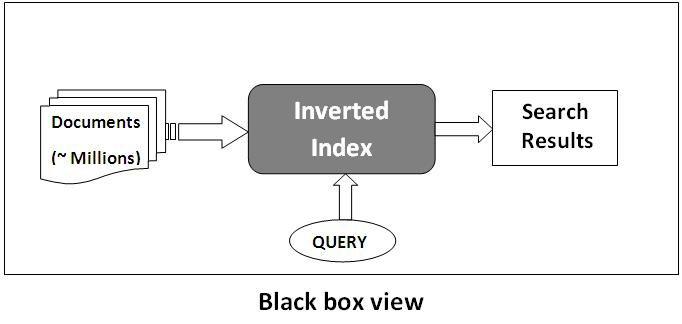
\includegraphics[width=\textwidth,height=!]{blackbox}
  \end{center}
  \caption{A black-box view of the indexer}
  \label{fig:blackbox}
\end{figure} 


\begin{figure}
  \begin{center}
	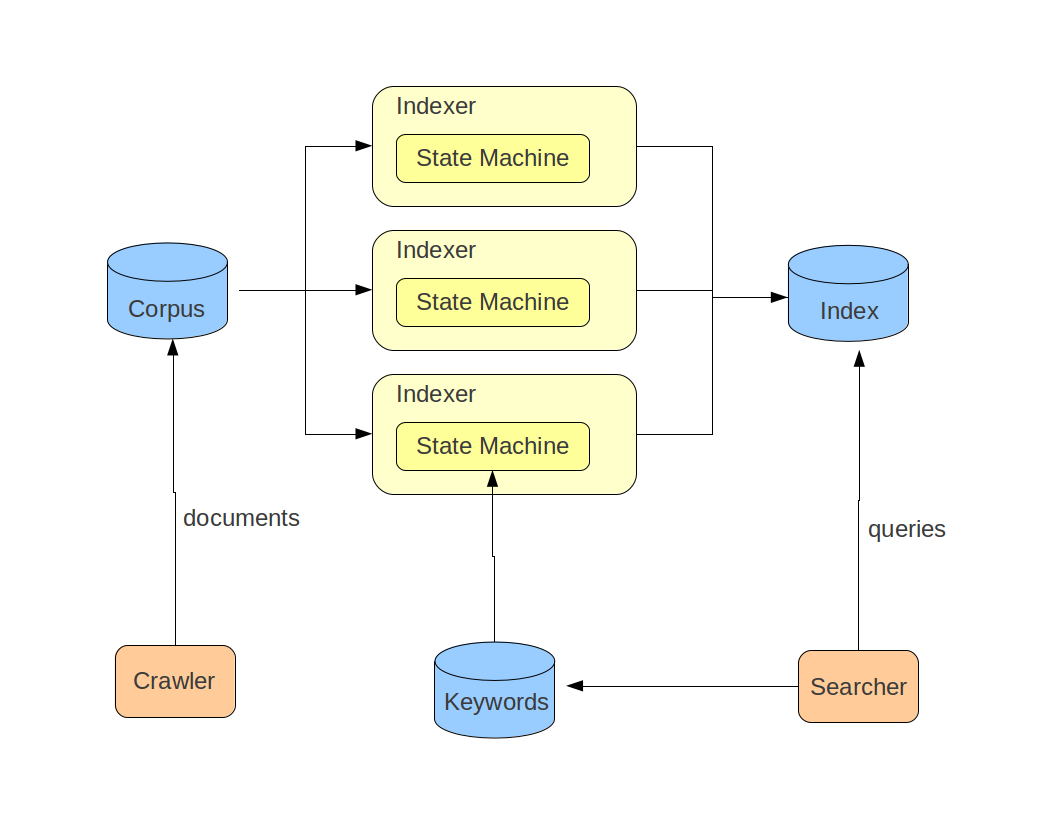
\includegraphics[width=\textwidth,height=!]{deploymentmodel}
  \end{center}
  \caption{Indexer deployment model}
  \label{fig:deploymentmodel}
\end{figure} 

A guiding architectural principal of the indexer design is to separate the implementation
into three logical layers:
\begin{itemize}
\item \textbf{Software Layer:} implements parsing, indexing and search
  algorithms.
\item \textbf{Data Access Layer:} implements an
  \textit{object-relational mapping}, insulating algorithm
  implementation from the persistence details. This layer implements
  classes which encapsulate persistent entities within the system.
\item \textbf{Database:} the persistent store for the document
  collection and inverted index.
\end{itemize}

The implementation classes and their relationships are represented in
a UML class diagram in figure \ref{fig:overallclassdiagram}. Figure
\ref{fig:overallsequencediagram} is a UML sequence diagram showing how
the layers interact at a high level.  The implementation of each of
these layers is described in more detail in section
\ref{sec:implementation}.

\begin{figure}
  \begin{center}
	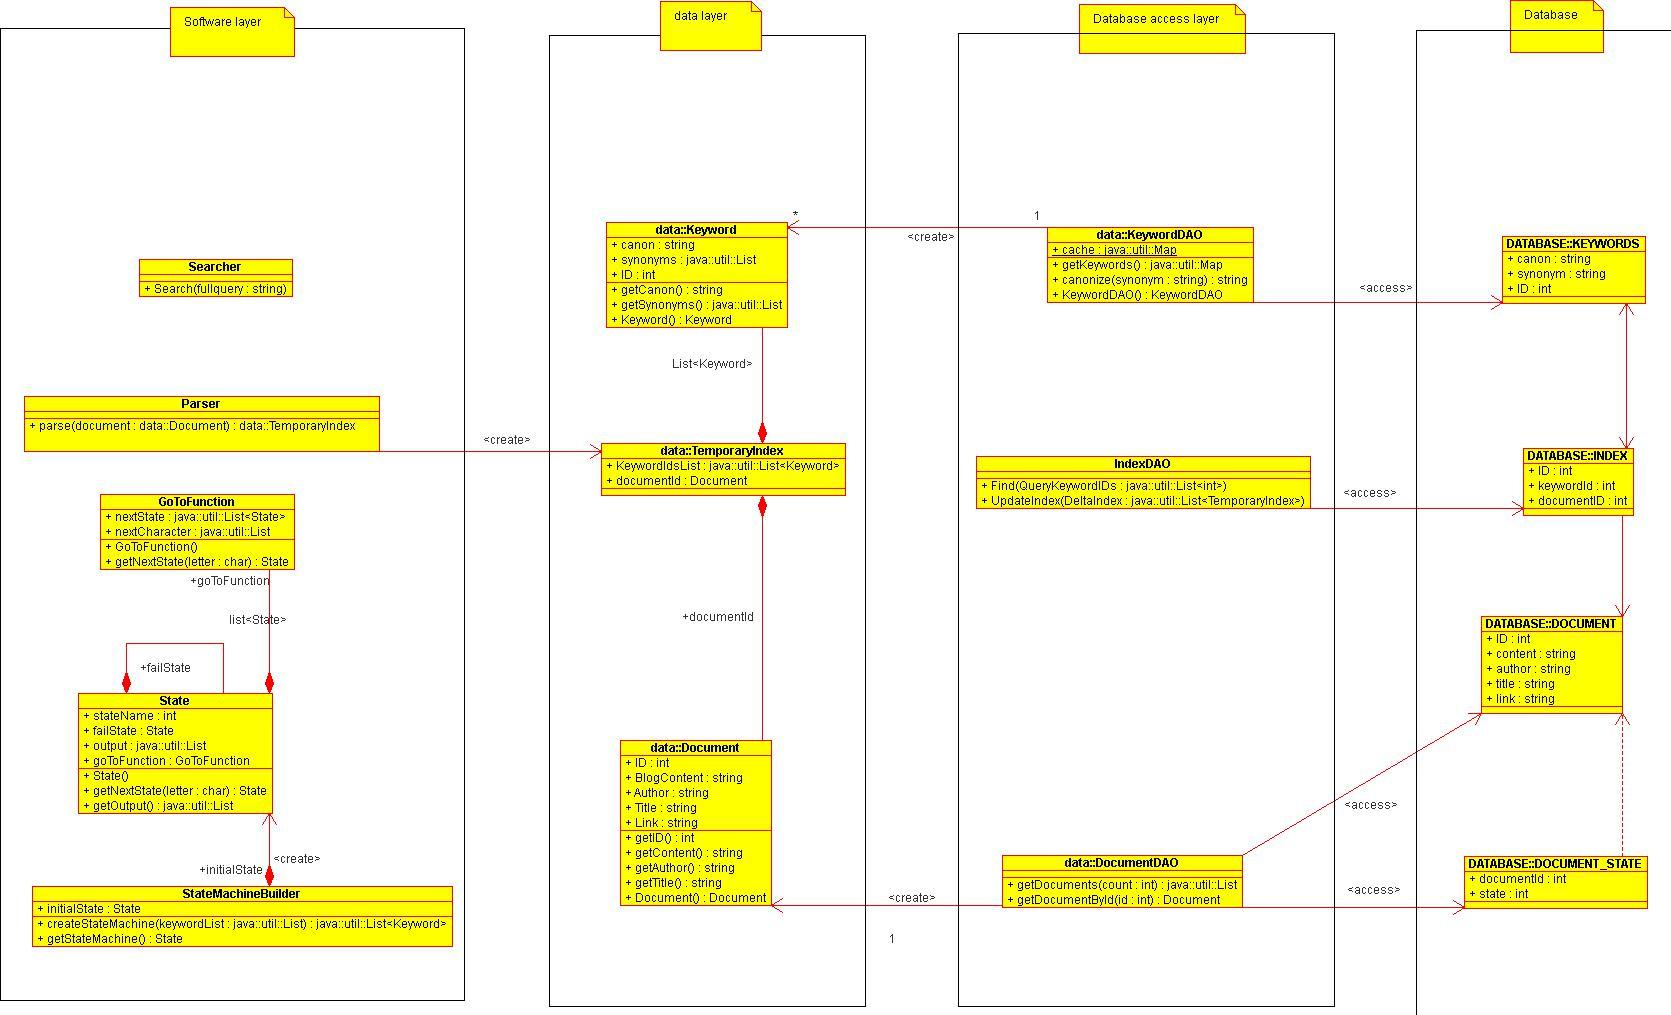
\includegraphics[width=\textwidth,height=!]{overallclassdiagram}
  \end{center}
  \caption{Overall UML class diagram design}
  \label{fig:overallclassdiagram}
\end{figure} 

\begin{figure}
  \begin{center}
	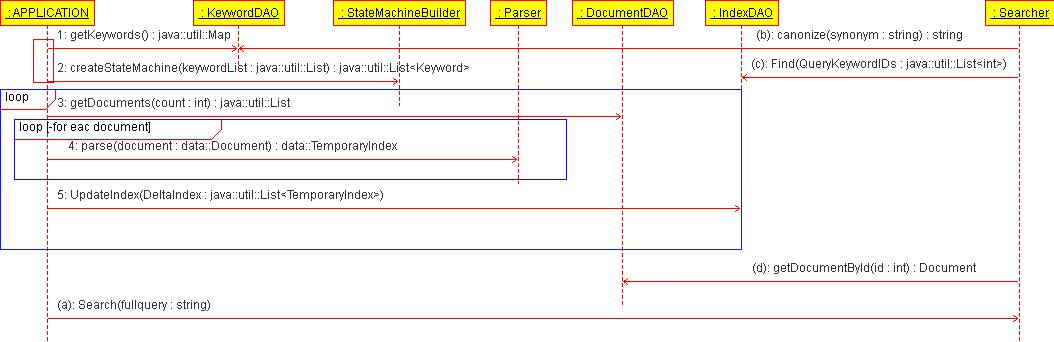
\includegraphics[width=\textwidth,height=!]{overallsequencediagram}
  \end{center}
  \caption{Overall UML sequence diagram design}
  \label{fig:overallsequencediagram}
\end{figure} 


%----------------------------------------
% Implementation 
%----------------------------------------
\section{Implementation}
\label{sec:implementation}
The individual worker processes of the indexer system are implemented as Java
programs. The programs make use of the following thirdparty libraries:

\begin{itemize}
  \item \textbf{DBPool:} a database connection pooling library, used
    to manage connections to relational databases.
  \item \textbf{Apache Commons Logging:} a generic logging API used by
    DBPool.
  \item \textbf{Apache Commons CLI:} a library for parsing command
    line arguments passed to Java programs.
  \item \textbf{MySQL JDBC driver:} the MySQL Java client driver.
\end{itemize}


The indexer system maintains an \textit{inverted index} of an evolving
corpus and services concurrent search requests against the index. The
current implementation is based on boolean retrieval methods described
in \cite{RefWorks:109}. An Aho-Corasick state machine
\cite{RefWorks:103} is used to scan documents for a predefined set of
keywords, and construct a term index for each document (delta
index). The term occurrences for each document are used to augment an
existing index for documents already processed. The document
collection, index, and keyword list are maintained in a single MySQL
database instance. It is through this database that the parallel
indexer instances are initialized and synchronized. This configuration
is operationally simple and easy to implement but the database has the
potential to become a throttle point as the system is scaled to larger
and faster-evolving document collections, and is required to service a
higher rate of queries. In order to scale the current implementation
to large document collections, a more efficient mechanism would be
required in this respect.

The following subsections detail the implementation of the
architectural layers identified in section \ref{sec:designcomponent}.

% Data Access Layer
\subsection{Data Access Layer}
\label{sec:dataaccesslayer}
Access to persistent storage is via objects of the data access
layer. Confining data access to a logical grouping of classes
insulates the other application components from changes in database
schema. The following subsections detail the individual data entities
handled by the data access later.


% Document
\subsubsection{Document}
\label{sec:document}
The \texttt{DocumentDAO} singleton class provides methods for retrieving
\texttt{Document} objects from the document database: 

\begin{itemize}
\item \texttt{List<Document> getDocuments (int count)}: retrieve a
  specified number of unprocessed documents from the database. The
  documents retrieved will be atomically marked as processed so that
  processing is not duplicated on other nodes. In this scheme, a
  document is considered processed to all other processes once
  retrieved from the database. This may cause problems from a fault
  recovery perspective if the processing node fails. A proposed
  enhancement to this scheme is to use another state, processing, to
  indicate that the document has been retrieved and to update the
  state to a processed state once processing is actually complete. For
  the initial implementation we will use the processed state only.

\item \texttt{Document getDocumentById (int id)}: retrieve a specific
  document from the database, referenced by its ID. 

\item \texttt{int getID ()}: accessor method.
\item \texttt{String getContent ()}: accessor method.
\item \texttt{String getAuthor ()}: accessor method.
\item \texttt{String getTitle ()}: accessor method
\item \texttt{String getLink()}: accessor method.
\end{itemize}

The \texttt{Document} class encapsulates the BLOG database table, with the
addition of a state field that tracks whether a document has been
processed or not. Figures \ref{fig:documentclassdiagram} and
\ref{fig:documentsequencediagram} show class and sequence diagrams
respectively for non-trivial classes and methods involved in the
implementation of the Document data access layer. 

\begin{figure}
  \begin{center}
	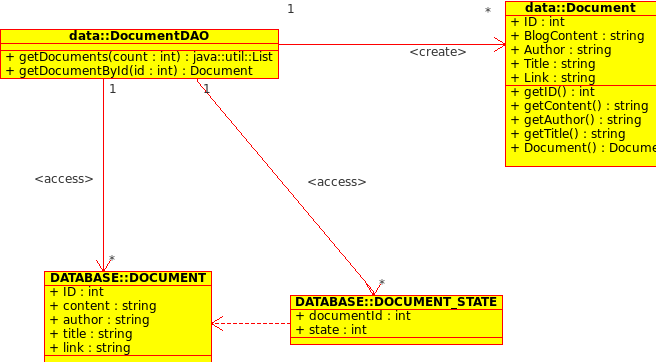
\includegraphics[width=\textwidth,height=!]{documentclassdiagram}
  \end{center}
  \caption{Document class diagram}
  \label{fig:documentclassdiagram}
\end{figure} 

\begin{figure}
  \begin{center}
	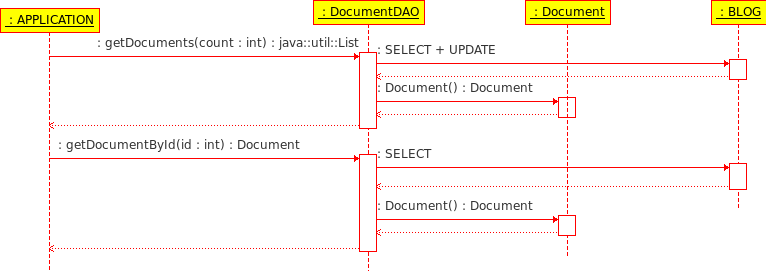
\includegraphics[width=\textwidth,height=!]{documentsequencediagram}
  \end{center}
  \caption{Document sequence diagram}
  \label{fig:documentsequencediagram}
\end{figure} 


% Keyword
\subsubsection{Keyword}
The \texttt{KeywordDAO} singleton class provides methods for
retrieving \texttt{Keyword} objects from the document
database. Because the keyword set is relatively static and accessed
often, the full set of keywords will be loaded from the database and
cached when the class initializes. The class also provides methods for
converting search terms to their canonical form.

\begin{itemize}
\item \texttt{List<String> getKeywords ()}: this method
  will returns a list of all \texttt{Keyword} objects defined in the
  keyword database. 

\item \texttt{List<Integer> canonize (String query)}: return the list
  of IDs corresponding to a comma-separated list of query terms.

\item \texttt{Keyword getKeywordById (int id)}: return the
  \texttt{Keyword} object with the given identifier.
\end{itemize}

The \texttt{Keyword} field encapsulates a canonical search term and a
list of its synonyms. Figures \ref{fig:keywordclassdiagram} and
\ref{fig:keywordsequencediagram} show UML class and sequence diagrams
respectively for non-trivial classes and methods involved in the
implementation of the Keyword data access layer. 

\begin{figure}
  \begin{center}
	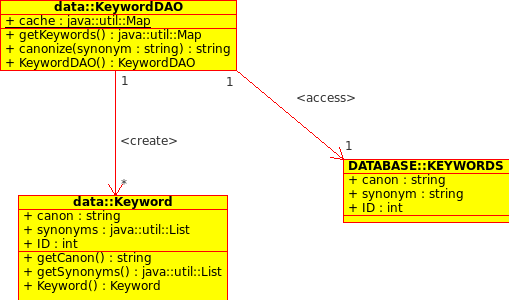
\includegraphics[width=\textwidth,height=!]{keywordclassdiagram}
  \end{center}
  \caption{Keyword class diagram}
  \label{fig:keywordclassdiagram}
\end{figure} 

\begin{figure}
  \begin{center}
	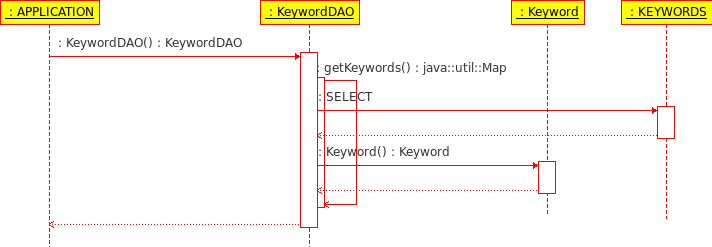
\includegraphics[width=\textwidth,height=!]{keywordsequencediagram}
  \end{center}
  \caption{Keyword sequence diagram}
  \label{fig:keywordsequencediagram}
\end{figure} 


% Index
\subsubsection{Index}
The \texttt{IndexDAO} class provides methods for updating and
searching the inverted index table stored in the database. There are
two methods defined in this class: 

\begin{itemize}
\item \texttt{void UpdateIndex (List<TempIndex> input)}: this method
  takes input of type List<TempIndex> (Note: Temporary index is a user
  defined data class, which contains Document ID and List of <keyword
  ids> as its attributes) and generates an SQL query which updates the
  INDEX table in the Database. 

\item \texttt{List<Integer> Find (List<Integer> QueryKeywordIds)}:
  this method takes a list of \texttt{Integers} (which corresponds to
  mapped \texttt{String} query into keyword ids) as input and searches
  the INDEX table in DB to find all the document ids which are common
  between for the given query keywords. 
\end{itemize}

 Figures \ref{fig:indexclassdiagram} and
 \ref{fig:indexsequencediagram} shows the UML class and sequence
 diagrams respectively for classes and methods involved in the
 implementation of the Index data access layer.

\begin{figure}
  \begin{center}
	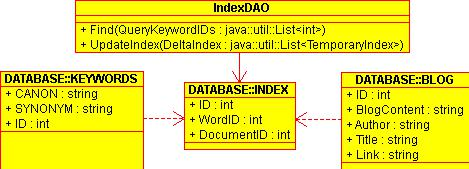
\includegraphics[width=\textwidth,height=!]{indexclassdiagram}
  \end{center}
  \caption{Index class diagram}
  \label{fig:indexclassdiagram}
\end{figure} 

\begin{figure}
  \begin{center}
	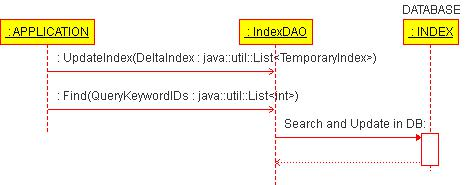
\includegraphics[width=\textwidth,height=!]{indexsequencediagram}
  \end{center}
  \caption{Index sequence diagram}
  \label{fig:indexsequencediagram}
\end{figure} 


% Software Layer
\subsection{Software Layer}

% Searcher
\subsubsection{Searcher}
This class is designed to perform searches for a query entered by the
user. It contains a method named \texttt{search ()} which is responsible for
finding all the documents which contained all query keywords.

\begin{itemize}
\item \texttt{List<Document> search (String)}: given a comma-separated
  list of search terms, returns the list of documents in which
  the canonical form of all search terms appear together. This method
  First calls \texttt{List<int> KeywordDAO.canonize (String)}, to map
  string query keywords into corresponding list of keyword IDs.  Note:
  We are assuming that the query will be formed with the set of
  keywords, which will be a subset of the global keyword set, with which
  the parsing state machine is constructed.

  Then it calls \texttt{List<Integer> IndexDAO.find (List<querykeywordIDs>)},
  which will searches in INDEX DB for a list of Common DOC\_IDs
  corresponding to given query keywords. 

  In the end, it calls \texttt{List<Document>
    DocumentDAO.getDocumentById (DOC\_ID)}. This will map DOC\_ID into
  a \texttt{Document} from the BLOG table in the database.  
\end{itemize}
 
Figures \ref{fig:searcherclassdiagram} and
\ref{fig:searchersequencediagram} shows the UML class and sequence
diagrams respectively for classes and methods involved in the
implementation of the \texttt{Searcher} class.


\begin{figure}
  \begin{center}
	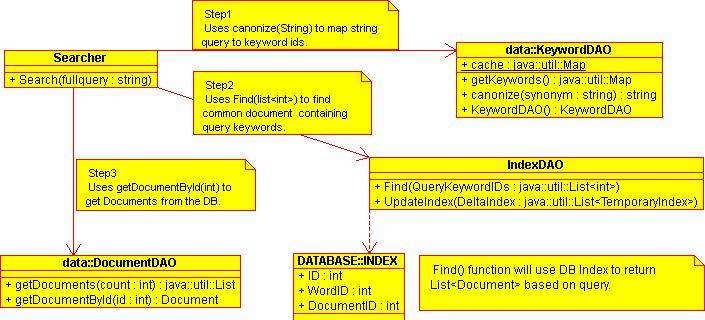
\includegraphics[width=\textwidth,height=!]{searcherclassdiagram}
  \end{center}
  \caption{Searcher class diagram}
  \label{fig:searcherclassdiagram}
\end{figure} 

\begin{figure}
  \begin{center}
	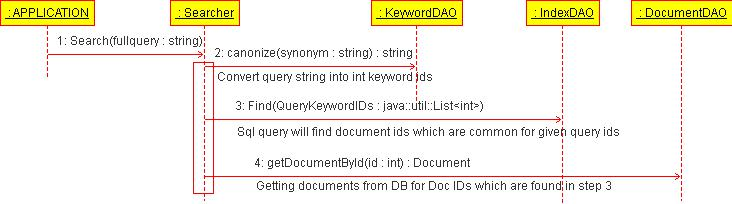
\includegraphics[width=\textwidth,height=!]{searchersequencediagram}
  \end{center}
  \caption{Searcher sequence diagram}
  \label{fig:searchersequencediagram}
\end{figure} 


% State Machine
\subsubsection{State Machine}
This class is designed to build the state machine from the list of
keywords returned by the \texttt{KeywordDAO.getKeywords()} method. This class has a static
attribute \texttt{initialState} that is the first state of the state machine
built by the function \texttt{createStateMachine} (initializes with the value
null). The first state gives us the whole state machine thanks to the
architecture of a state. Once the state machine is built, the function
\texttt{getStateMachine} is used to access the initial state stored in the
class.

Figures \ref{fig:statemachineclassdiagram} and
\ref{fig:statemachinesequencediagram} shows the UML class and sequence
diagrams respectively for classes and methods involved in the
implementation of the \texttt{StateMachineBuilder}.

\begin{figure}
  \begin{center}
	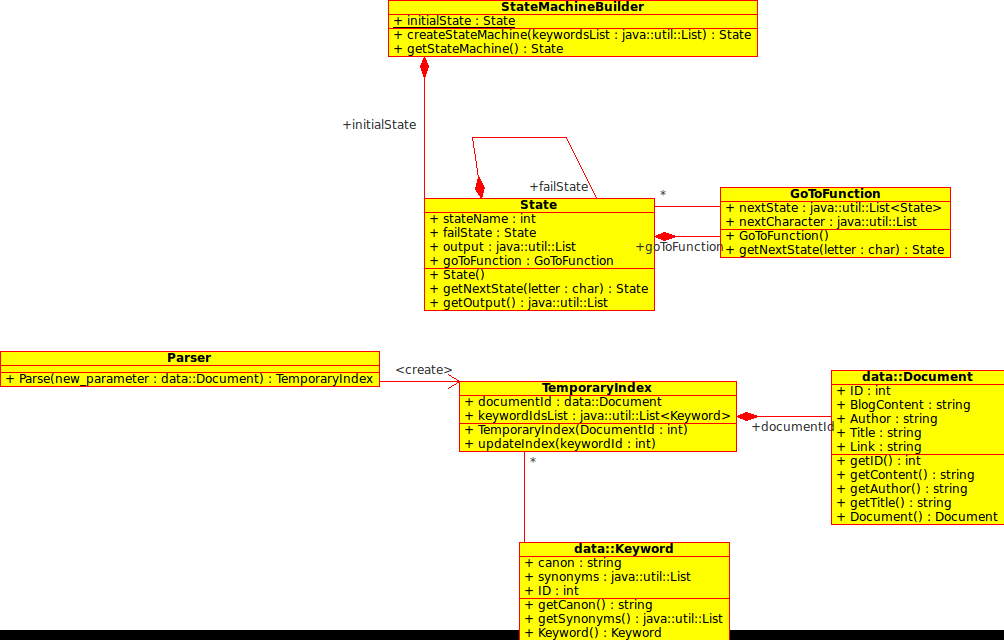
\includegraphics[width=\textwidth,height=!]{statemachineclassdiagram}
  \end{center}
  \caption{State machine class diagram}
  \label{fig:statemachineclassdiagram}
\end{figure} 

\begin{figure}
  \begin{center}
	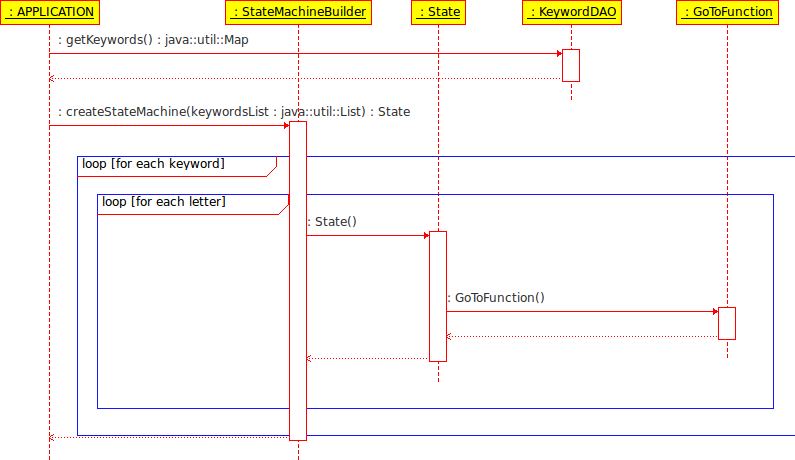
\includegraphics[width=\textwidth,height=!]{statemachinesequencediagram}
  \end{center}
  \caption{State machine sequence diagram}
  \label{fig:statemachinesequencediagram}
\end{figure} 


% Parser
\subsubsection{Parser}
The \texttt{Parser} implements the document parsing algorithm within
the state machine. By default, it uses the state machine contained
in the static attribute of \texttt{StateMachineBuilder}. To parse a
document we need to call the \texttt{parse ()} function inside this
class, passing it the \texttt{Document} class encapsulating the actual
text we want to parse. This class returns a \texttt{TemporaryIndex}
object which encapsulates a reference to the document parsed and the
keywords found to occur within the document.

Figures \ref{fig:parserclassdiagram} and
\ref{fig:parsersequencediagram} shows the UML class and sequence
diagrams respectively for classes and methods involved in the
implementation of the \texttt{Parser}.

\begin{figure}
  \begin{center}
	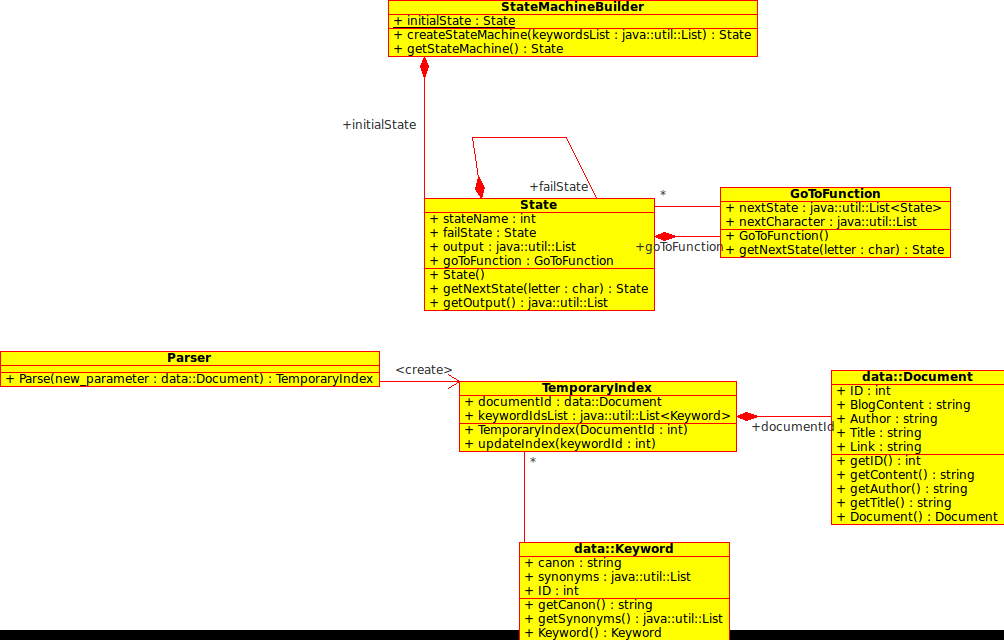
\includegraphics[width=\textwidth,height=!]{parserclassdiagram}
  \end{center}
  \caption{Parser class diagram}
  \label{fig:parserclassdiagram}
\end{figure} 

\begin{figure}
  \begin{center}
	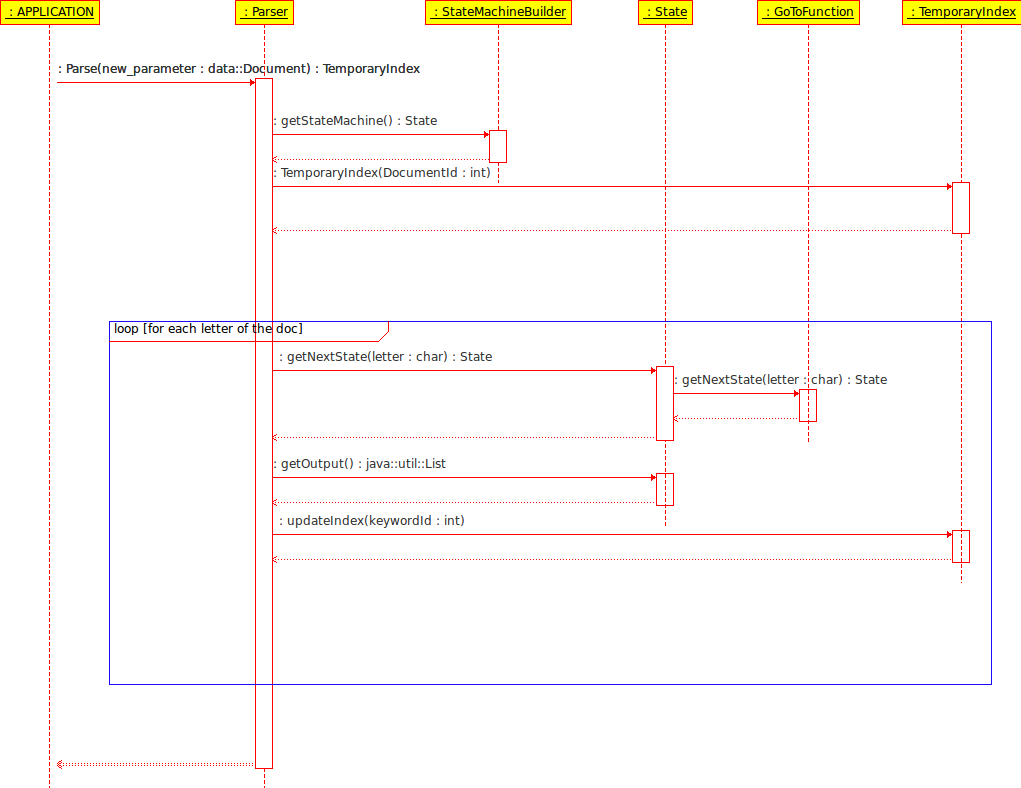
\includegraphics[width=\textwidth,height=!]{parsersequencediagram}
  \end{center}
  \caption{Parser sequence diagram}
  \label{fig:parsersequencediagram}
\end{figure} 


%----------------------------------------
% Experiment Results
%----------------------------------------
\section{Experiment Results}
\label{sec:experimentresults}
FIX: All tests were run on a Dell laptop with an Intel Core Duo 2GHz
processor, 1GB RAM, running a 32 bit Linux 2.6.37 kernel. The Java
Virtual Machine used was version 1.6.0-24.....


%----------------------------------------
% Conclusions
%----------------------------------------
\section{Conclusions}
\label{sec:conclusions}


%----------------------------------------
% Bibliography
%----------------------------------------
% Change Bibliography title to 'References'
\renewcommand\bibname{References}
\bibliography{bibliography}
\bibliographystyle{IEEEannot}


%--------------------------------------------------
\end{document}
